%%%%%%%%%%%%%%%%%%%%%%%%%%%%%%%%%%%%%%%%%%%%%%%%%%%%%%%%%%%%%%%%%%%%%%%%
%    INSTITUTE OF PHYSICS PUBLISHING                                   %
%                                                                      %
%   `Preparing an article for publication in an Institute of Physics   %
%    Publishing journal using LaTeX'                                   %
%                                                                      %
%    LaTeX source code `ioplau2e.tex' used to generate `author         %
%    guidelines', the documentation explaining and demonstrating use   %
%    of the Institute of Physics Publishing LaTeX preprint files       %
%    `iopart.cls, iopart12.clo and iopart10.clo'.                      %
%                                                                      %
%    `ioplau2e.tex' itself uses LaTeX with `iopart.cls'                %
%                                                                      %
%%%%%%%%%%%%%%%%%%%%%%%%%%%%%%%%%%
%
%
% First we have a character check
%
% ! exclamation mark    " double quote  
% # hash                ` opening quote (grave)
% & ampersand           ' closing quote (acute)
% $ dollar              % percent       
% ( open parenthesis    ) close paren.  
% - hyphen              = equals sign
% | vertical bar        ~ tilde         
% @ at sign             _ underscore
% { open curly brace    } close curly   
% [ open square         ] close square bracket
% + plus sign           ; semi-colon    
% * asterisk            : colon
% < open angle bracket  > close angle   
% , comma               . full stop
% ? question mark       / forward slash 
% \ backslash           ^ circumflex
%
% ABCDEFGHIJKLMNOPQRSTUVWXYZ 
% abcdefghijklmnopqrstuvwxyz 
% 1234567890
%
%%%%%%%%%%%%%%%%%%%%%%%%%%%%%%%%%%%%%%%%%%%%%%%%%%%%%%%%%%%%%%%%%%%
%
\documentclass[12pt]{iopart}
\newcommand{\gguide}{{\it Preparing graphics for IOP Publishing journals}}
%Uncomment next line if AMS fonts required
%\usepackage{iopams} 



\usepackage{graphicx}           % Import Pictures + PDFs
\usepackage[svgnames]{xcolor}   % Enabling colors by their 'svgnames'
\definecolor{fzjblue}{HTML}{005B81}
\definecolor{light-gray}{gray}{0.97}
\definecolor{mygreen}{rgb}{0,0.6,0}
\usepackage{listings} %  See: https://en.wikibooks.org/wiki/LaTeX/Source_Code_Listings
\lstset{
  language=Python,
  backgroundcolor=\color{light-gray},   % choose the background color; you must add \usepackage{color} or \usepackage{xcolor}
  basicstyle=\linespread{1}\footnotesize,        % the size of the fonts that are used for the code
  commentstyle=\color{mygreen},
  frame=single,
  keywordstyle=\color{blue},       % keyword style
  tabsize=4,	                   % sets default tabsize to 2 spaces
  rulecolor=\color{light-gray},
}

\newcommand{\python}[0]{\texttt{Python} }
\newcommand{\abs}[1]{\left\vert #1 \right\vert}

\begin{document}

\title[A primer to numerical simulations]{A primer to numerical simulations: The perihelion
motion of Mercury}

\author{I. Hammer, C. Hanhart, C. K\"orber and C. M\"uller}

\address{Forschungszentrum J\"ulich}
\ead{c.hanhart@fz-juelich.de}
\vspace{10pt}
%\begin{indented}
%\item[]February 2014
%\end{indented}

\begin{abstract}
Numerical simulations are playing an increasingly important role in modern science. In this work it is
suggested to use a numerical study of the famous perihelion motion of the planet Mercury (one of the prime observables
supporting Einsteins General Relativity) as a test case to teach numerical simulations to high school students.
The paper includes details about the development of the code as well as a discussion of the visualization 
of the results. In addition a method is discussed how to estimate the size of the effect a priori. 
\end{abstract}

% Uncomment for PACS numbers
%\pacs{00.00, 20.00, 42.10}
%
% Uncomment for keywords
%\vspace{2pc}
%\noindent{\it Keywords}: XXXXXX, YYYYYYYY, ZZZZZZZZZ
%
% Uncomment for Submitted to journal title message
%\submitto{\JPA}
%
% Uncomment if a separate title page is required
%\maketitle
% 
% For two-column output uncomment the next line and choose [10pt] rather than [12pt] in the \documentclass declaration
%\ioptwocol
%



\section{Introduction}

Numerical simulations play a key role in modern physics for they allow one to tackle theoretical problems
not accessible otherwise, e.g., since there are too many particle participating in the system (as in
simulations for weather predictions) or the interactions are too complicated to allow for a systematic,
perturbative approach (as in theoretical descriptions of nuclear particles at the fundamental level). 
 The goal of this paper is it to
introduce a project that could be used to make numerical simulations themselves the topic of the class.
On the example of the perihelion motion of the planet Mercury the students are supposed to get in touch with
\begin{itemize}
\item the importance of differential equations in theoretical physics;
\item the numerical implementation of Newtonian dynamics;
\item systematic test and optimization of computer codes;
\item effective tools to estimate the result a priori as an important cross check;
\item the visualization of numerical results using V-Phython.
\end{itemize}
The course as well as this paper is structured as follows: after an introduction to Newtonian dynamics and the 
concepts of differential equations their discretization is discussed based on Newtons law of gravitation and possible
extensions thereof. Afterwards the visualization of the resulting trajectories using V-Phython is introduced and
applied to the problem at hand. In particular tools are developed to extract the relevant quantity from the result
of the simulation.
Finally the principle of dimensional analysis is presented as a tool to cross check, if the results of the simulation
are sensible.

\section{Trajectories, velocities, accelerations and Newtons second law}
\label{sec:tva}

We can say that we understand a physical system if we can demonstrate that an assumed force leads to the trajectories
observed, where here trajectory means that we can calculate the location in space of the object of interest at any point
in time, once the initial conditions are fixed properly. If we can neglect the finite size of this object the location is parametrized
by a single three vector $\vec x(t)$. As will become clear below in order to describe and control the dynamics of a physical
object in addition we need to be able to calculate its velocity, $\vec v(t)$, related to the location via
\begin{equation}\label{eq:x_update}
\vec x(t+\Delta t) = \vec x(t) + \vec v(t) \Delta t + ... \ , \label{eq:vdef}
\end{equation}
for some infinitesimally small $\Delta t$ and the acceleration, $\vec a(t)$ that describes the change of the velocity
\begin{eqnarray}\label{eq:v_update}
\vec v(t+\Delta t) = \vec v(t) + \vec a(t) \Delta t + ...\ . \label{eq:adef}
\end{eqnarray}
The dots in the above expressions indicate that there are in general additional terms that may be expressed with
higher powers in $\Delta t$, however, for sufficiently small $\Delta t$ those can be safely neglected.
Thus we may define the time derivative via
\begin{equation}
\vec v(t) = \lim_{\Delta t\to 0} \frac{\Delta \vec x(t)}{\Delta t} =: \frac{d\vec x(t)}{dt}  = \dot{\vec  x}(t) \ ,
\end{equation}
where $\Delta \vec x(t)=\vec x(t+\Delta t)-\vec x(t)$ and we introduced with the last expression a common short hand notation
for time derivatives. Analogously we get
\begin{eqnarray}
\vec a(t) &=& \lim_{\Delta t\to 0} \frac{\Delta \vec v(t)}{\Delta t} =: \frac{d\vec v(t)}{dt}  = \dot{\vec v}(t) \ , \\
 &=& \frac{d^2\vec x(t)}{dt^2}  = \ddot{\vec x}(t) \ ,
\end{eqnarray}
where we introduced in the second line the second derivative.

It was Newton who observed that if a body is at rest it will remain at rest, and if it is in motion it will remain in motion in a 
constant velocity in a straight line, unless it is acted upon by some force --- this is known as Newtons first law. 
Said differently: a force $\vec F$shows up by changing the motion of some object. This is quantified in Newton's second law
\begin{equation}
\vec F(\vec x, t) = \frac{d}{dt}(m \vec v) \ .
\end{equation} 
If the mass does not change~\footnote{A well known example where $m$ does change with time is a 
rocket, whose mass decreases as the rocket rises.} with time this reduces to the well known
\begin{equation}
\vec F(\vec x) = m \vec a(t) = m\dot{\vec v}(t) = m\ddot{\vec{x}}(t) \ . \label{eq:newton2}
\end{equation} 
Note that in general the force could depend also on the time or the velocity, we here restrict ourselves to the
case relevant for our example where the force depends on the location only. 
Therefore, 
as soon as the force $\vec F(\vec x)$ is known for all $\vec x$ one can in principle can, e.g., Eq.~(\ref{eq:newton2})
for $\vec x(t)$.
Sometimes requires some advanced knowledge in math, sometimes no closed form solution exists. However, alternatively 
one can calculate the whole trajectory
of some test body that experiences this force by a successive application of the rules 
given in Eqs.~(\ref{eq:vdef}) and (\ref{eq:adef}):
\begin{enumerate}
\item For a given time $t$, where $\vec x(t)$ and $\vec v(t)$ are known, use Eq.~(\ref{eq:newton2}) to calculate $\vec a(t)$.
\item Use Eq.~(\ref{eq:vdef}) to calculate $\vec x(t+\Delta t)$ and
\item then use Eq.~(\ref{eq:adef}) to calculate $\vec v(t+\Delta t)$.
\item Go back to (i).
\end{enumerate}
Clearly to initiate the procedure at some time $t_0$ both $\vec x(t_0)$ as well as $\vec v(t_0)$ must be known --- the 
trajectories depend on these initial conditions.~\footnote{In general a differential equation of $n^{\rm th}$ degree (where
the highest derivative is $n$) needs $n$ initial conditions specified. For $n=2$ those are often chosen as location and velocity
at some defined time, but also to pick two location at different times is possible. }

Clearly for this procedure to work $\Delta t$ must be sufficiently small. What this means depends on the process
studied. One way to check, if $\Delta t$ is small enough is to verify, if the realation
\begin{equation}
\vec v(t) \gg \frac12\vec a(t)\Delta t
\label{eq:check}
\end{equation}
holds, for the next term neglected in Eq.~(\ref{eq:vdef}) reads $(1/2)a(t)(\Delta t)^2$.  Eq.~({\ref{eq:check}})
also shows that small (large) time steps are necessary (sufficient), if the force is strong (weak), since
the time steps need to be small enough that all changes induced by the force get resolved.



\section{Example: The perihelion motion of Mercury}


For this concrete example the starting point for the force is Newtons law
of gravitation
\begin{equation}
F_N(\vec x) = \frac{G_N m M_\odot}{r^2} \ ,
\end{equation}
where $G_N=6.67\times 10^{-11}$ m$^3$kg$^{-1}$s${-2}$ is the Newtonian constant of gravitation,
$m$ is the mass of Mercury and $M_\odot=2\times 10^{30}$ kg is the mass of the sun.
In addition $r=|\vec x(t)|$ denotes the distance between sun and Mercury, when we assume that the sun
is infinitely more heavy than the planet and located at the center of the coordinate system. Although this is not exact, since $m/M_\odot\sim 10^{-8}$ this is
a pretty good approximation. For later convenience we introduce the Schwarzschildradius of the sun
\begin{equation}
r_S=\frac{2G_N  M_\odot}{c^2} = 3 \ \mbox{km} \ ,
\end{equation}
where $c=3\times 10^8$ m/s denotes the speed of light.
With this Newtons second law reads 
\begin{equation}
\ddot{\vec x} = \frac{c^2}{2}\left(\frac{r_S}{r^2}\right) \ .
\label{eq:newton}
\end{equation}
\begin{itemize}
\item{\bf First task:}
Now the students should implement the program outlined in Sec.~\ref{sec:tva} and visualize the resulting
trajectories of Mercury for different start parameters.
Why is it sufficient to work in two dimensions using simply 
$\vec x(t)=(x(t),y(t))^T$?
 When the parameters are chosen appropriately close
orbits should emerge that are fixed in time --- in particular the perihelion (the point of closest approach
of planet and sun) stays fixed in space.
\end{itemize}
It is a well known feature of a $1/r^2$ force that elliptic orbits with fixed perihelion emerge. However, as soon
as the potential is different, the perihelion moves. This will be studied next:
\begin{itemize}
\item{\bf Second task:}
Now the students should add a new term to the right hand side of Eq.~(\ref{eq:newton}). In particular the equation should now
read 
\begin{equation}
\ddot{\vec x} = \frac{c^2}{2}\left(\frac{r_S}{r^2}\right)\left(1+\alpha\left(\frac{r_S}{r}\right)\right) \ ,
\label{eq:newton_art}
\end{equation}
where $\alpha$ is some parameter. What happens to the trajectories as $\alpha$ is varied?
\end{itemize}
Finally the start values need to be chosen appropriately such that the simulation indeed mimicks the trajectories
of Mercury ...


\section{Numerical Implementation}
In this section we present the numerical implementation of the perihelion motion of Mercury.  We select \python as the programming language of choice \cite{}, because \python is easy to learn, intuitive to understand and an open source language\footnote{See also appendix \ref{appendix:python} for an instruction how to set up python on different operating systems.}.  No prior knowledge of \python or any other programming language is required because we explain all the essential steps in order to create the simulation.  We also provide a working example \cite{} which can be used as template.

The first step of a numerical simulation is the extraction of the relevant physical parameters and quantities in order to translate the problem to mathematical equations.  The relevant objects for this example are the sun and mercury.  Thus, to describe their motion, one needs their "initial" distances, velocities and accelerations which are the input to their equation of motions (Eq.~(\ref{eq:x_update}) and Eq.~(\ref{eq:v_update})).  In the case of this problem, one can simplify the implementation by placing one planet (the "infinitely" heavy sun) in the center of the coordinate system and describe the motion of the other planet (mercury) in a two-dimensional plane.  \textit{Why is this simplified picture sufficient to describe the motion}?

Because the problem does not depend on the initial position of mercury on its orbit around the sun, we extract the parameters at the perihelion with $ \abs{\vec r_{MS}(0)} = 46 \cdot 10^6 km$ and $ \abs{\vec v_M(0)} = 39 km/s $\footnote{https://nssdc.gsfc.nasa.gov/planetary/factsheet/mercuryfact.html}.  Since the computer does not understand physical units, one has to express each variable in their respective unit.  Both, for the numerical treatment and the intuitive understanding, it is useful to select parameters in a "natural range".  A particular useful choice for this problem is given by expressing time intervals in days $T_0 = 1d$ and distances in $R_0 = 10^{10}m$.  With this choice, the initial distance of mercury to the sun, the initial velocity of mercury and the acceleration prefactor become
\begin{equation}
	r_{MS}(0) = 4.6 R_0 \, , \quad
	v_{M}(0)  = 0.34 \frac{R_0}{T_0} \, ,  \quad
	a_M       = 0.99 \frac{R_0}{T_0^2} \frac{1}{\left(r_{MS}/R_0\right)^2}
	\, .
\end{equation}

\begin{figure}[htb]
	\centering
	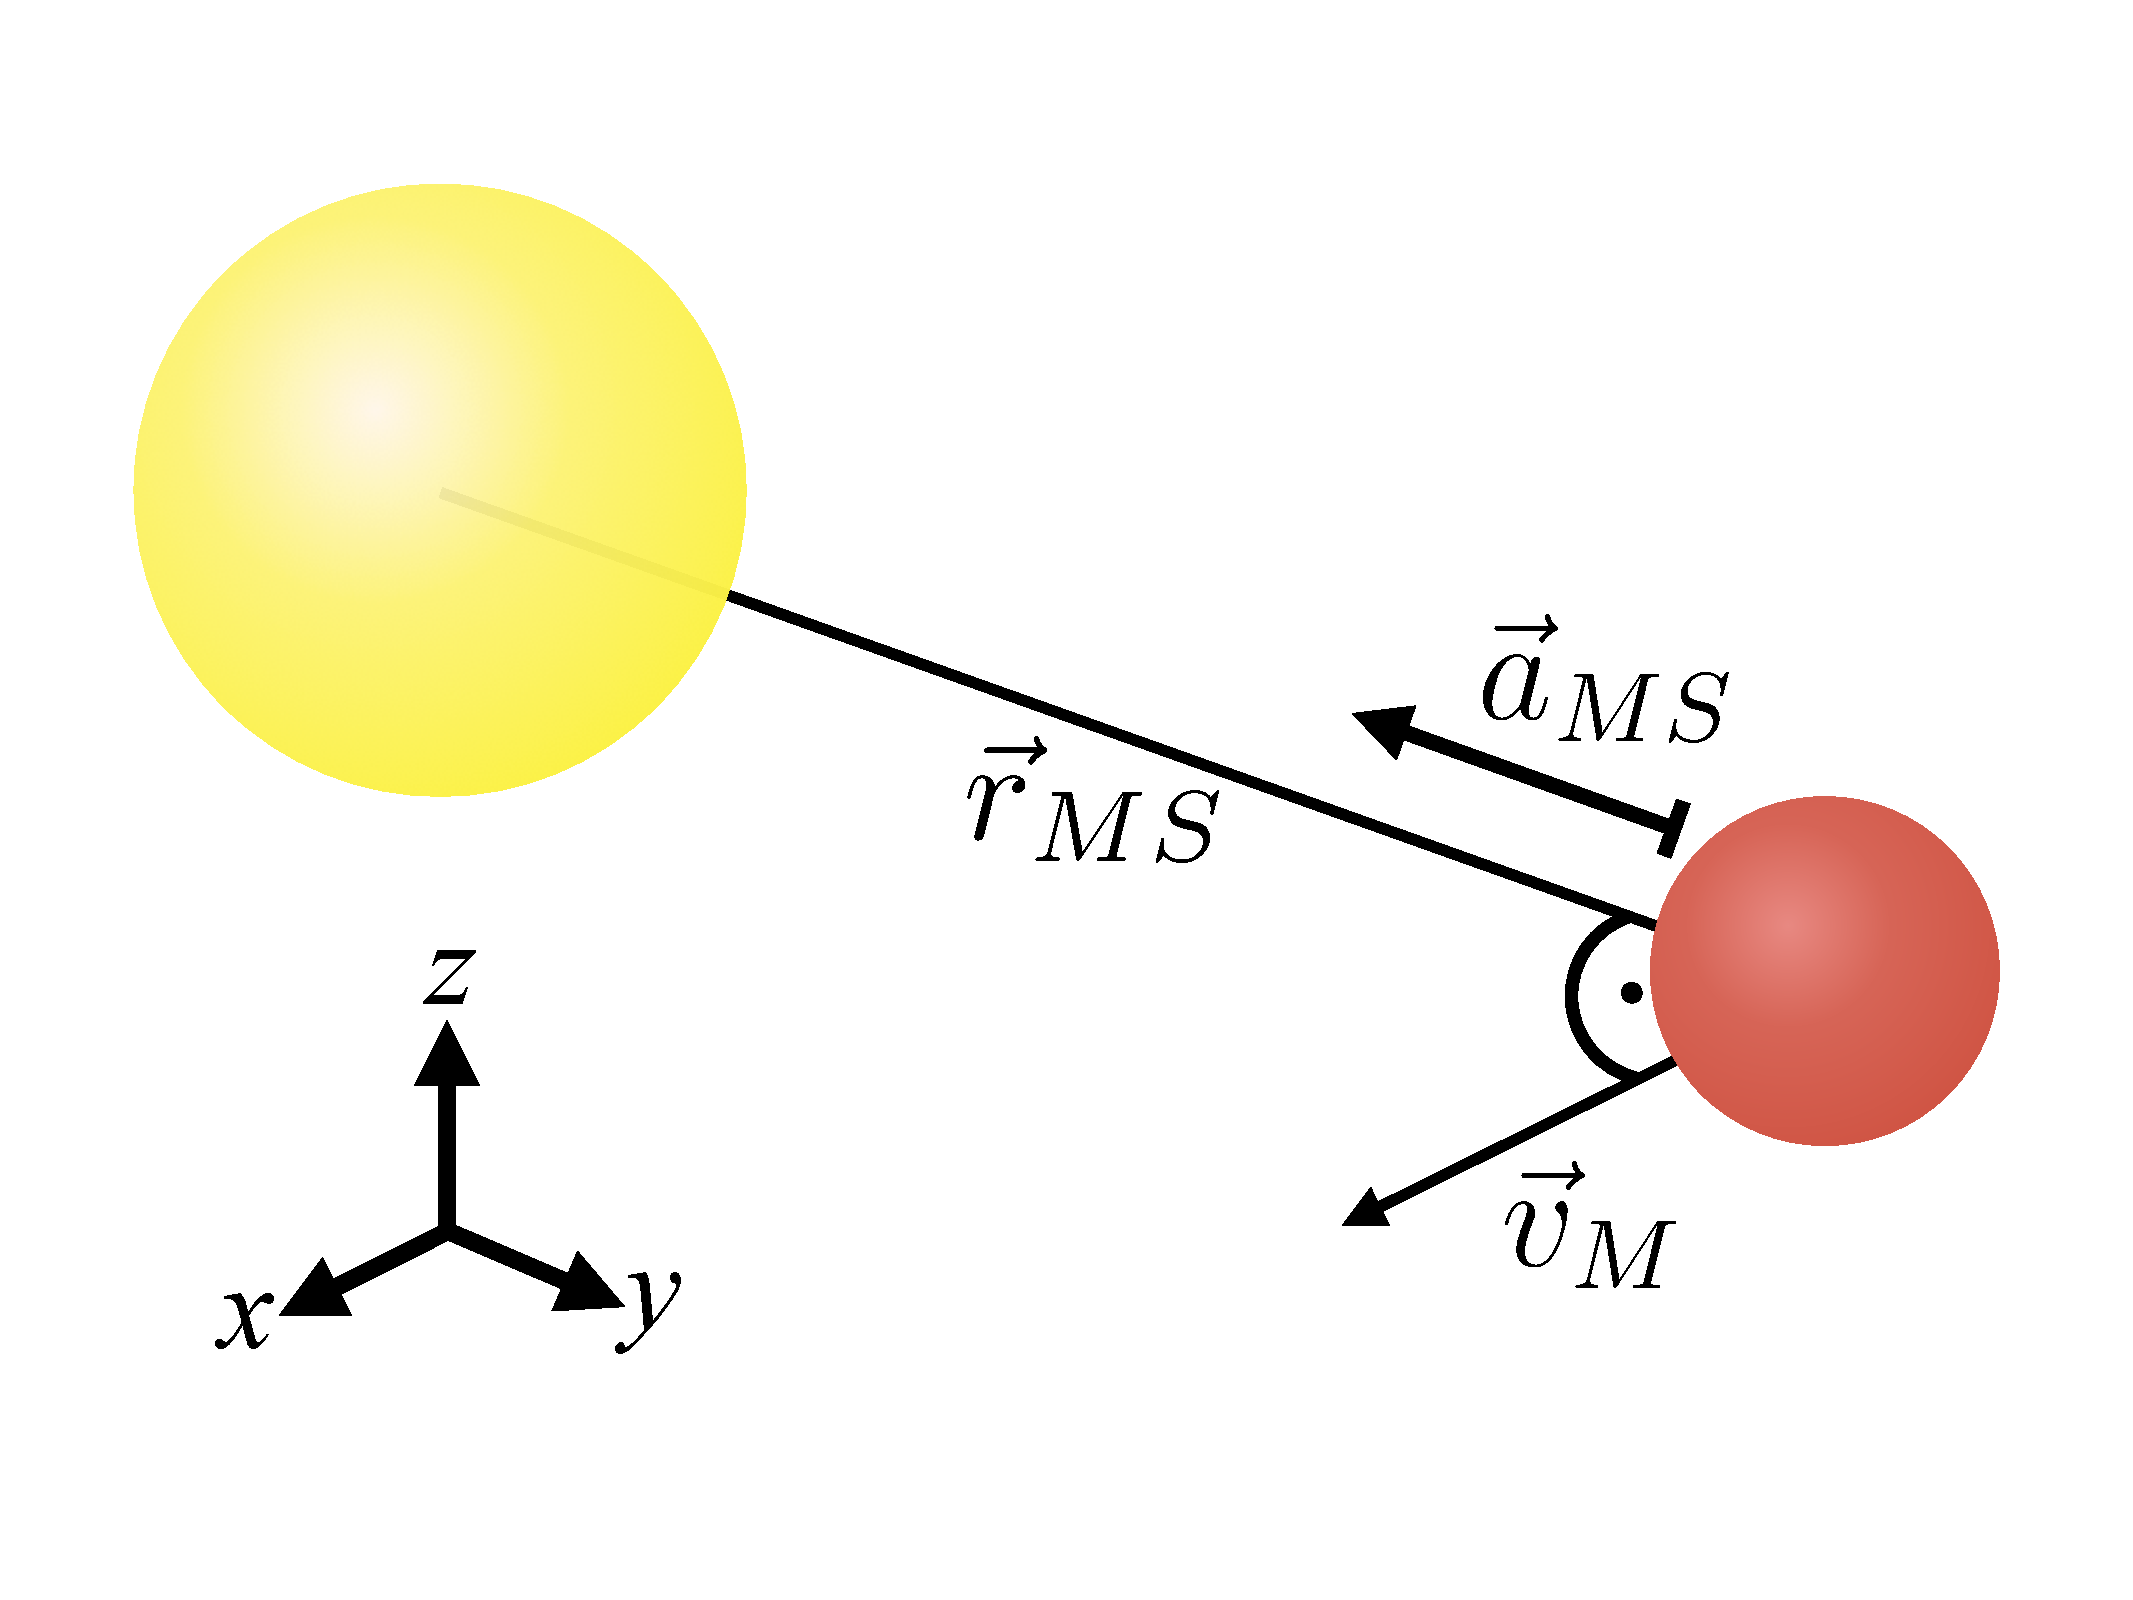
\includegraphics[width=.4\textwidth]{figs/sun_merc.pdf}
	\caption{\label{fig:sun_merc}Sun mercury system with relevant vectors.  Because the mercury is at its perihelion, its velocity is perpendicular to its direct connection vector with the sun.}
\end{figure}


In python, this reads
\begin{lstlisting}
	# Definition of parameters
	rM0 = 4.6    # in units of R0
	vM0 = 0.34   # in units of R0/T0
	aM  = 0.99   # in units of R0/T0**2
\end{lstlisting}
Next, we set up the initial vectors which will describe the motion in the two-dimensional plane.  We will build on the existing \python module: \texttt{Vpython}, which provides implementation for the vectorial implementation and animation.  The first object of interest is a \texttt{vector}, which takes three-dimensional coordinates as its input.  Because of our choice of initial conditions, the velocity of mercury is perpendicular to the vector which connects mercury and the sun (see figure \ref{fig:sun_merc}):
\begin{lstlisting}
	# Import the class vector from python
	from vpython import vector
	# Initialize distance and velocity vectors
	vec_rS0 = vector(0, 0, 0)
	vec_rM0 = vector(0, rM0, 0)
	vec_vM0 = vector(vm0, 0, 0)
\end{lstlisting}
According to Eq.~(\ref{eq:newton}), the force which acts on mercury changes the velocity of mercury which eventually changes the position.  In first approximation we can numerically express the updates of the position and the velocity by
\begin{lstlisting}
	# Compute the strength of the acceleration
	aMS = aM * ( 1 + alpha * rS / vec_rM_old.mag  ) / vec_rM_old.mag**2
	# Multiply by the direction
	vec_aMS = - aMS * ( vec_rM_old / vec_rM_old.mag )
	# Update velocity vector
	vec_vM_new = vec_vM_old + vec_aMS * dt
	# Update position vector
	vec_rM_new = vec_rM_old + vec_vM_new * dt
\end{lstlisting}
Note the beauty of working with the predefined \texttt{vector} class: the basic vector operations are already implemented.  The difference and sum of two vectors, or the scalar vector multiplication return vectors themselves.  Also the magnitude of a vector -- \texttt{vector.mag} -- is a property of the vector and can be easily extracted.

It is handy to use \texttt{Python}s \texttt{function}s to embed repeating structures ("DRY" -- Don't Repeat Yourself)
\begin{lstlisting}
	# Define the function
	def evolve_mercury(vec_rM_old, vec_vM_old):
		<...Code...>
		return vec_rM_new, vec_vM_new
	
	# Call the function
	vec_rM_new, vec_vM_new = do_time_step(vec_rM_old, vec_vM_old)
\end{lstlisting}
Because of \python{}s syntax, it is necessary that the body of the function is indented relative to the definition statement.

Finally, we can express the evolution by a \texttt{while}-loop
\begin{lstlisting}
	t = 0
	# Execute the loop as long as t < T
	while t < T:
		vec_rM, vec_vM = evolve_mercury(vec_rM, vec_vM)
		t = t + dt
\end{lstlisting}
Note the required indent of the loop structure similar to the indent of a function.  In each iteration of the \texttt{while}-loop, the previous distance and velocity are used to compute the new values -- which directly overwrite the previous values and thus enter the next iteration. The time step \texttt{dt} needs to be sufficiently small in order to avoid numerical errors.  We recommend $dt = ...$.  The total runtime \texttt{T} is the amount of "virtual" days the simulations should run.  To describe at least one full orbit, $T$ needs to be larger than $T>..$.


Ideas for questions:
\begin{itemize}
	\item Mass and motion of sun
	\item Estimate \texttt{dt} and also \texttt{T} in order to cover roughly two "mercury years".
	\item What does happen when you change those units?
	\item Compare values to the values in \cite{}.  Where does the difference come from?
	\item Start with $\alpha=0$. What do you observe?
\end{itemize}

\section{Visualization using V-Phython}

\section{Dimensional analysis}

Dimensional analysis is not only a tool that allows one to cross check if the results of some simulation is
of the right order of magnitude, it is also very helpful to identify unusual dynamics in some system.
Especially the latter aspect should become clear from the discussion in this section.

The idea of dimensional analysis is that in a system that can be controlled by expanding the relevant quantities
(like the force) in some small parameter(s), the coefficients in the expansion should turn out to be of order unity (that
means anything between about 0.1 and 10 is fine - but 0.01 or 100 is irritating) --- parameters in line with this
are called 'natural'. Applied to the problem at hand
given by Eq.~(\ref{eq:newton}) this statement implies that from naturalness one would expect that 
the parameter $\alpha$ is of order 1 when one uses
for $r$ the average distance Mercury-sun, namely $\bar r=6\times 10^7$ km.
Form this one estimates for the expected angular shift per orbit
\begin{equation}
\delta \phi \simeq 2\pi\left(\frac{r_S}{\bar r}\right) = (\pi \times 10^{-7}) \ \mbox{rad} = (2\times 10^{-5})^o = (7\times 10^{-2}) ^{''} \ ,
\end{equation}
which leads to a shift of  about $30^{''}$ in 100 earth years to be compared to the empirical value of $43^{''}$.
 Thus indeed the
amount of perihelion motion of Mercury is in line with expectations, $if$ --- and this is an important 'if' ---
the Newtonian dynamics is simply the leading term of some more general underlying theory. In particular,
no new scales enter in the correction terms.

Thanks to Einstein we indeed know that the conclusion formulated above is correct ---- the more general underlying
theory is General Relativity and indeed Einstein was able to quantitatively explain the perihelion motion of Mercury
from his equations. 
On the other hand had we found a dramatic deviation of $\alpha$ from unity one would have concluded that 
there is probably some other dynamics going on that drives this difference.

Indeed, we now several of those hierarchy problems in modern physics: e.g. the so called QCD $\theta$ term,
expected to be of natural size, is at present known to be at most $10^{-10}$. This smallness, called the
strong CP problem, is so irritating that physicists like S. Weinberg even proposed that there must exist an
additional particle, the axion, whose interactions are in charge of pushing $\theta$ even to zero and there
are now intense searches for this axion going on various labs.

\section{Summary and possible extensions}

%\begin{table}
%\caption{\label{jlab1}Journals to which this document applies, and macros for the abbreviated journal names in {\tt iopart.cls}. Macros for other journal titles are listed in appendix\,A.}
%\footnotesize
%\begin{tabular}{@{}llll}
%\br
%Short form of journal title&Macro name&Short form of journal title&Macro name\\
%\mr
%2D Mater.&\verb"\TDM"&Mater. Res. Express&\verb"\MRE"\\
%\br
%\end{tabular}\\
%$^{a}$UK spelling is required; $^{b}$MSC classification may be used as well as PACS; $^{c}$titles of articles are required in journal references; $^{d}$Harvard-style references must be used (see section \ref{except}); $^{e}$final page numbers of articles are required in journal references.
%
%\end{table}
%\normalsize



\subsection{Acknowledgments}
Here they come

\appendix
\section{Instructions to install V-phython}
\label{appendix:python}

\section{The code}
Here we should put the code
 

\bibliographystyle{plain}
\bibliography{MercuryNumerical}

\end{document}

